
\documentclass[conference]{article}
\usepackage[margin=1in]{geometry}
\usepackage{cite}
\usepackage{amsmath,amssymb,amsfonts}
\usepackage{algorithmic}
\usepackage{graphicx}
\usepackage{textcomp}
\usepackage{xcolor}
\usepackage{subcaption}

\begin{document}
	\section{Steady State Model}
	The circuit to be analyzed is the continuous conversion ratio circuit as seen in \cite{Butzen2019}, which can be seen in Fig. \ref{fig:contTop}. The various steps are numbered along with their associated capacitors in Fig. \ref{fig:contTop}, and will be used further in the analysis. The circuit diagram corresponding to a single flying capacitor and its switches (also referred to as a "core") can be seen in Fig. \ref{fig:coreCon}. The initial analysis and modeling is performed under the following assumptions,
	\begin{itemize}
		\item All the capacitors are linear.
		\item The top and bottom plate parasitic capacitance's have minimal impact on the transient and steady state characteristics of the converter, and are neglected from the analysis.
		\item All the flying capacitors are equally sized with capacitance $C_{Fly}$, where $C_{Fly} = C_{1,0} = C_{1,1} = C_{2,0} = C_{2,M} ...$
		\item The switches for the intermediary nodes, $S_{T1}, S_{T2}, S_{TM}, S_{B1}, S_{BN}, etc$, all have an equivalent resistance $R_{ON}$. The resistance of the switches which connect to the positive and negative rails is 0 ($S_{T+}, S_{T-}, S_{B+}, S_{B-}$).
	\end{itemize}
	\begin{figure}
		\centering
		\includegraphics[width=0.7\linewidth]{Figures/contRatioCircuit2.pdf}
		\caption{Circuit diagram illustrating the various connections made by the flying capacitors for the continuous ratio.}
		\label{fig:contTop}
	\end{figure}
	\begin{figure}
		\centering
		\includegraphics[width=0.4\linewidth]{Figures/contRatioCore.pdf}
		\caption{Circuit diagram illustrating the top and bottom connections of a single flying capacitor.}
		\label{fig:coreCon}
	\end{figure}
	\subsection{Charge Transfer Analysis}
	The operation of the converter is as follows, each capacitor iterates from steps (1,0)$\rightarrow$(4,M) sequentially. There is always a connection to either 0, $V_{IN}$ or $V_{OUT}$ through one of the large interconnection switches, which act as shorts due to their 0$\Omega$ resistance. The other connection to the intermediary voltage domains occurs through a switch with a resistance $R_{ON}$, where the core voltage begins to equalize with the new voltage domain. An example circuit can be seen in Fig. \ref{fig:step_Circ1}, which is electrically equivalent to Fig. \ref{fig:step_Circ2}. 
	
	\begin{figure}
		\centering
		\begin{subfigure}{0.4\textwidth}
			\centering
			\includegraphics{Figures/step2_Circ.pdf}
			\caption{Circuit configuration including switches and flying capacitors.}
			\label{fig:step_Circ1}
		\end{subfigure}
		\begin{subfigure}{0.4\textwidth}
			\centering
			\includegraphics{Figures/step2_Eq.pdf}
			\caption{Equivalent circuit with values.}
			\label{fig:step_Circ2}	
	\end{subfigure}
		\caption{Example circuit diagrams showing the connection to $B_1$.}
	\end{figure}

	\begin{figure}
		\centering
		\includegraphics[width=0.7\linewidth]{Figures/V-(t).pdf}
		\caption{Illustration of $V_{-}(t)$ for various time steps over the period, where $V_-$ is the bottom plate of the capacitor, as in \ref{fig:step_Circ1}.}
		\label{fig:V-(t)}
	\end{figure}
	
	The circuit diagram in Fig. \ref{fig:step_Circ2}, can be used to calculate the transient response of the circuit over each time step. As both the flying capacitance and resistance of each core is identical, the voltage at the intermediary node ($B_N$) is constant over the time step. This is a result of the symmetry in impedance on either side of the node. The resulting $RC$ time constant will be referred to as $\tau$, where 
	\begin{equation}
	\tau = R_{ON}C_{Fly}.
	\end{equation} 
	This time constant can be used to describe the change in voltage with respect to time, as the capacitors connect to different voltage domains. Take the existing example as in Fig. \ref{fig:step_Circ2}, the top plate voltages are known, while the bottom plate voltage of $C_{1,1}$ ($V_{1,1}^{-}$) can be calculated as,
	\begin{equation}
	V_{-}^{1,1}(t) = V_{OUT}\exp\left(\frac{-t}{\tau}\right) + V_{BN}\left(1-\exp\left(\frac{-t}{\tau}\right)\right),
	\end{equation}
	where $t$ is the time after the start of the step. More generally, the top and bottom plate voltages can be described as,
	\begin{equation}
	V_{C}[n] = V_{C}[n-1]\exp\left(\frac{-t}{\tau}\right) + V_{int}\left(1-\exp\left(\frac{-t}{\tau}\right)\right),
	\label{eq:Vstepn}}
	\end{equation}
	where the voltage at $V_{C}[n-1]$ is the voltage at the end of previous step, while $V_{int}$ is the voltage of the intermediary node ($V_{T1}$, $V_{TM}$, $V_{B1}$, etc) which the capacitor is connected to. Next, the duration of each time step can be incorporated into the analysis, using the switching frequency ($f_{SW}$). A substitution can then be made to simplify the analysis, where
	\begin{equation}
	A = 1-\exp\left(\frac{-1}{\tau f_{SW}}\right),
	\end{equation}
	which can be substituted into (\ref{eq:Vstepn}) for example
	\begin{equation}
		V_{C}[n] = V_C[n-1]A + V_{int}(1-A),
	\end{equation}
	which can then be used to express the bottom plate voltage as a series of multiplications. The bottom plate voltage for steps (1,1)$\rightarrow $(1,N) is illustrated in Fig. \ref{fig:V-(t)}, and can be described as a sequence of transitions, where
	\begin{equation}
	\begin{split}
	V_-^{1,1} &= V_{OUT}(1-A) + AV_{BN},\\
	V_-^{1,2} &= V_-^{1,1}(1-A) + AV_{BN-1},\\
	& \,\,\,\vdots\\
	V_{-}^{1,N} &= V_-^{1,N-1}(1-A) + AV_{B1}.
	\end{split}		
	\end{equation}
	Using this, a matrix can be constructed to describe the bottom plate voltages,
	\begin{equation}
	\begin{split}
	\begin{bmatrix}
	V_-^{1,1} \\
	V_-^{1,2} \\
	\vdots\\
	V_-^{1,N-1} \\ 
	V_-^{1,N}
	\end{bmatrix}
	&\!=\!
	\begin{bmatrix}
	A \!& 0 & \dots & 0 & 0 \\
	A(1-A) \!& A & \dots & 0 & 0\\
	\vdots & \vdots & \ddots & \vdots & \vdots \\
	A(1\!-\!A)^{N-2} \!& A(1\!-\!A)^{N-3} \!& \dots & A & 0\\ 
	A(1\!-\!A)^{N-1} \!& A(1\!-\!A)^{N-2} \!& \dots & A(1-A) & A 
	\end{bmatrix}\!\begin{bmatrix}
	V_{BN} \\
	V_{BN-1} \\
	\vdots \\
	V_{B2} \\
	V_{B1}
	\end{bmatrix}\\&+V_{OUT}\begin{bmatrix}
	(1-A) \\
	(1-A)^2 \\
	\vdots \\
	(1-A)^{N-1} \\
	(1-A)^N
	\end{bmatrix}.
	\end{split}
	\label{eq:V-Matrix}
	\end{equation}
	Using a similar method, a matrix can be constructed for the bottom plate voltages in steps (3,N)$\rightarrow$(3,1),
	\begin{equation}
	\begin{split}
	\begin{bmatrix}
	V_-^{3,N} \\
	V_-^{3,N-1} \\
	\vdots\\
	V_-^{3,2} \\ 
	V_-^{3,1}
	\end{bmatrix}
	&\!=\!
	\begin{bmatrix}
	A \!& A(1-A) & \dots & A(1\!-\!A)^{N-2} & A(1\!-\!A)^{N-1} \\
	0 \!& A & \dots & A(1\!-\!A)^{N-3} \! & A(1\!-\!A)^{N-2}\\
	\vdots & \vdots & \ddots & \vdots & \vdots \\
	0 \!&  0& \dots & A & A(1-A) \\ 
	0 \!& 0 \!& \dots & 0 & A 
	\end{bmatrix}\!\begin{bmatrix}
	V_{BN} \\
	V_{BN-1} \\
	\vdots \\
	V_{B2} \\
	V_{B1}
	\end{bmatrix}\\
	\end{split}.
	\end{equation}
	Next, a charge balance analysis can be used to calculate the current moving into and out of nodes $B_1 \rightarrow B_N$ on each time step. In both cases, the charge into the node can be calculated using the change in voltage on the capacitor,
	\begin{equation}
	Q_{Bx} = C_{Fly}(V_-^{1,x} - V_-^{1,x-1}),
	\end{equation}
	where $x$ is the index from 1 to $N$. This can be used to construct matrices for both steps $(1,1)\rightarrow(1,N)$ .
	\begin{equation}
	\begin{bmatrix}
	Q_{BN} \\
	Q_{BN-1} \\
	\vdots\\
	Q_{B2} \\ 
	Q_{B1}
	\end{bmatrix}
	=
	\begin{bmatrix}
	-A \!& 0 & \dots & 0 & 0 \\
	A^2 \!& -A & \dots & 0 & 0\\
	\vdots & \vdots & \ddots & \vdots & \vdots \\
	A^2(1\!-\!A)^{N-3} \!& A^2(1\!-\!A)^{N-4} \!& \dots & -A & 0\\ 
	A^2(1\!-\!A)^{N-2} \!& A^2(1\!-\!A)^{N-3} \!& \dots & A^2 & -A 
	\end{bmatrix}\!\begin{bmatrix}
	V_{BN} \\
	V_{BN-1} \\
	\vdots \\
	V_{B2} \\
	V_{B1}
	\end{bmatrix}\!C\\+CV_{DD}\begin{bmatrix}
	A \\
	A(1-A) \\
	\vdots \\
	A(1-A)^{N-2} \\
	A(1-A)^{N-1}
	\end{bmatrix},
	\end{equation}
	and $(3,1)\rightarrow(3,N)$ 
	\begin{equation}
	\begin{bmatrix}
	Q_{BN} \\
	Q_{BN-1} \\
	\vdots\\
	Q_{B2} \\ 
	Q_{B1}
	\end{bmatrix}
	=
	\begin{bmatrix}
	-A \!& A^2 & \dots & A^2(1\!-\!A)^{N-3} & A^2(1\!-\!A)^{N-2} \\
	0 \!& \!-A & \dots & A^2(1\!-\!A)^{N-4} & A^2(1\!-\!A)^{N-3}\\
	\vdots & \vdots & \ddots & \vdots & \vdots \\
	0 \!& 0 \!& \dots & -A & A^2\\ 
	0 \!& 0 \!& \dots & 0 & -A 
	\end{bmatrix}\!\begin{bmatrix}
	V_{BN} \\
	V_{BN-1} \\
	\vdots \\
	V_{B2} \\
	V_{B1}
	\end{bmatrix}.
	\end{equation}
	The charge out of the nodes can then be added, and summed to zero, as the voltage at the nodes does not change at steady state. The resulting matrix is,
	\begin{equation}
	\begin{bmatrix}
	0 \\
	0 \\
	\vdots\\
	0 \\ 
	0
	\end{bmatrix} =
	CM\begin{bmatrix}
	V_{B1} \\
	V_{B2} \\
	\vdots \\
	V_{BM-1} \\
	V_{BM}
	\end{bmatrix} + \!CV_{DD}\begin{bmatrix}
	A \\
	A(1-A) \\
	\vdots \\
	A(1-A)^{N-2} \\
	A(1-A)^{N-1}
	\end{bmatrix}.
	\end{equation}
	where 
	\begin{equation}
	M=\begin{bmatrix}
	-2A \!& A^2 & \dots & A^2(1\!-\!A)^{N-3} & A^2(1\!-\!A)^{N-2} \\
	A^2 \!& \!-2A & \dots & A^2(1\!-\!A)^{N-4} & A^2(1\!-\!A)^{N-3}\\
	\vdots & \vdots & \ddots & \vdots & \vdots \\
	A^2(1\!-\!A)^{N-3} \!& A^2(1\!-\!A)^{N-4} \!& \dots & -2A & A^2\\ 
	A^2(1\!-\!A)^{N-2} \!& A^2(1\!-\!A)^{N-3} \!& \dots & A^2 & -2A
	\end{bmatrix}.
	\end{equation}
	The solved expression for voltage levels $V_{B1} \rightarrow V_{BN}$ is,
	\begin{equation}
	V_{Bx} = V_{OUT}\frac{A(x-1) + 1}{A(N-1) + 2},
	\end{equation}
	a similar procedure can be followed to acquire the voltage levels for $V_{T1} \rightarrow V_{TN}$,
	\begin{equation}
	V_{Tx} = V_{OUT} + (V_{IN} - V_{OUT})\frac{A(x-1) + 1}{A(N-1) + 2}\,.
	\end{equation}
	These can now be substituted into (\ref{eq:V-Matrix}) for example to acquire the solved expressions for $V_-$ for steps (1,1) $\rightarrow$ (1,N).
	The solved expressions for the top and bottom plate voltages are:
	\begin{equation}
	V_{-}^{1,x} = \frac{((N-x-1)A + 2)V_{OUT}}{A(N-1) + 2},
	\end{equation}
	\begin{equation}
	V_{+}^{2,x} = V_{OUT} + (V_{IN} -V_{OUT})\frac{(M-x-1)A + 2}{A(M-1) + 2},
	\end{equation}
	\begin{equation}
	V_{-}^{3,x} = \frac{xAV_{OUT}}{A(N-1) + 2},
	\end{equation}
	\begin{equation}
	V_{+}^{4,x} = V_{OUT} + \frac{xA(V_{IN} -V_{OUT})}{A(N-1) + 2}.
	\end{equation}
	In order to calculate the input and output currents of the converter, a charge balance method will be used. The charge delivered to the output can be observed from Fig. \ref{fig:contTop}, where it occurs on steps (1,0), (3,0)$\rightarrow$(3,N) and (4,1)$\rightarrow$(4,M). The charge transferred on the steps is as follows,
	\begin{equation}
	Q_{3,0} = C_{Fly}(V_+^{2,M} - V_{OUT}),
	\end{equation}
	\begin{equation}
	Q_{3,1} \rightarrow  Q_{3,N} = C_{Fly}V_{3,N},
	\end{equation}
	and
	\begin{equation}
	Q_{4,1} \rightarrow  Q_{1,0} = C_{Fly}(V_{IN} - V_{OUT}),
	\end{equation}
	resulting in a total output charge of 
	\begin{equation}
	\begin{split}
	Q_{OUT} &= Q_{3,0} + Q_{3,1} + Q_{4,1}\\
	Q_{OUT} &= C_{Fly}\frac{(2-A)(V_{IN} - V_{OUT})}{A(M-1) + 2} + C_{Fly}\frac{NAV_{OUT}}{A(N-1) + 2} + C_{Fly}(V_{IN} - V_{OUT}) \\ 
	Q_{OUT} &= C_{Fly}\left(\frac{(A(M-2) + 4)(V_{IN} - V_{OUT})}{A(M-1) + 2} + \frac{NAV_{OUT}}{A(N-1) + 2}\right).
	\end{split}
 	\end{equation}
 	A similar method can be used to acquire the input charge, occurring over steps (1,0) $\rightarrow$ (2,0),
 	\begin{equation}
 	\begin{split}
 	Q_{IN} &= C_{Fly}\left(V_{IN} - V_+^{4,M} + V_{OUT}\right) \\
 	Q_{IN} &= C_{Fly}\left(V_{IN} - V_{OUT} - \frac{MA(V_{IN} -V_{OUT})}{A(M-1) + 2} + V_{OUT}\right) \\
 	Q_{IN} &= C_{Fly}\frac{MAV_{OUT} + (2-A)V_{IN}}{A(M-1) + 2}
 	\end{split}
 	\end{equation}
 	The input and output charge can then be used in combination with the switching frequency to acquire the input and output power,
 	\begin{equation}
 	P_{IN} = V_{IN}f_{SW}C_{Fly}\frac{MAV_{OUT} + (2-A)V_{IN}}{A(M-1) + 2},
 	\label{eq:P_IN}
 	\end{equation}
 	
 	\begin{equation}
 	P_{OUT} = V_{OUT}f_{SW}C_{Fly}\left(\frac{(2-A)(V_{IN} - V_{OUT})}{A(M-1) + 2} + \frac{NAV_{OUT}}{A(N-1) + 2} + (V_{IN} - V_{OUT})\right),
 	\label{eq:P_OUT}
 	\end{equation}
 	finally, an expression for the conversion efficiency ($\eta$) can be constructed,
 	\begin{equation}
 	\eta = \frac{P_{OUT}}{P_{IN}} = \frac{V_{OUT}}{V_{IN}}\frac{(A(N-1) + 2){(A(M-2) + 4)(V_{IN} - V_{OUT})} + (A(M-1) + 2)NAV_{OUT}}{(A(N-1) + 2)(MAV_{OUT} + (2-A)V_{IN})}.
 	\end{equation}
 	The resulting calculation for the efficiency is then graphed and compared to some simulation results with ideal components, which can be seen in Fig. \ref{fig:Comp_VIn} and \ref{fig:Comp_A}. Fig \ref{fig:Comp_VIn} plots the efficiency in comparison to input voltage, while Fig. \ref{fig:Comp_A} plots efficiency in comparison to $A$.
 	
 	\begin{figure}
 		\begin{subfigure}{0.5\textwidth}
 			\includegraphics[width=\linewidth]{Figures/eta_VIn.pdf}
 			\caption{Comparison with constant $A = 1$ and $V_{OUT} = 1$.}
 			\label{fig:Comp_VIn}
 		\end{subfigure}
 	\begin{subfigure}{0.49\textwidth}
 		\includegraphics[width=\linewidth]{Figures/eta_A.pdf}
 		\caption{Comparison with constant $V_{IN} = 2.5$ and $V_{OUT} = 1$.}
 		\label{fig:Comp_A}
 	\end{subfigure}
 		\caption{Verification of the calculated efficiency. The simulations were setup to conform to the model assumptions.}
 	\end{figure}
 
 	\section{Steady State Model Usefulness}
 	The usefulness of the model is going to be dependent on how accurate the underlying assumptions are, these will now be discussed. 
 	\subsection{Flying Capacitor Linearity}
 	Provided the flying capacitors are made from MIM (Metal Insulator Metal) or MOM (Metal Oxide Metal) capacitors, the assumption of linearity should hold. Alternately, if the capacitors are MOS based, then there is likely some non-linearity which will impact the accuracy of the design. It should be noted that many of the techniques used to reduce parasitic capacitance have the additional impact of improving capacitor linearity \cite{}, \cite{}. Regardless, there is a need to do additional analysis to assess the impact of non-linearity on the model, and to incorporate that into the model.
 	
 	A simple first order approximation would be to assess the total amount of charge required to drive the capacitor from $0 \rightarrow V_{IN}$, as this dictates the total change in charge on the capacitor. This can then be used to approximate how the value of $C_{Fly}$ changes as a function of $V_{IN}$, which will impact the power density. 
 	
 	\subsection{Top and Bottom Plate Parasitic Capacitance}
 	Top and bottom plate parasitic capacitances can be expressed as $C_{\alpha_T}$, and $C_{\alpha B}$, as seen in Fig. \ref{}. They are related to the flying capacitance by the factor $\alpha T$ and $\alpha B$, where,
 	\begin{equation}
 	C_{\alpha T} = C_{Fly}\alpha_T,
 	\end{equation}
 	and
 	\begin{equation}
 	C_{\alpha B} = C_{Fly}\alpha_B.
 	\end{equation}
 	
 	The effect of $C_{\alpha T}$ is increased current flowing from the input to output. It delivers charge to the output on step (3,0), as $C_{\alpha T}$ discharges from $V_{+}^{2,M} \rightarrow V_{OUT}$. This results in a total amount of charge,
 	\begin{equation}
 	Q_{\alpha T} = C_{\alpha T}(V_{+}^{2,M} - V_{OUT}) = C_{Fly}\alpha_T\frac{(2 - A)(V_{IN} - V_{OUT})}{A(M-1) + 2},
 	\end{equation}
 	being delivered to the output. Similarly, on step (1,0) $C_{\alpha T}$ draws charge from the input as it is charged from ($V_{+}^{4,M}$) to $V_{IN}$, 
 	\begin{equation}
 	Q_{\alpha_T} = C_{\alpha T}(V_{IN} - V_{+}^{4,M}) = C_{Fly}\alpha_{T}\frac{(2 - A)(V_{IN} - V_{OUT})}{A(M-1) + 2}.
 	\end{equation}
 	
 	The effect of $C_{\alpha B}$ is a decrease in total output current. Consider step (4,0), where the bottom plate is charged from $V_-^{3,N}$ to $V_{OUT}$, requiring charge,
 	\begin{equation}
 	Q_{\alpha B} = C_{\alpha B}(V_{OUT} - V_{-}^{3,N}) = C_{Fly}\alpha_B\frac{V_{OUT}(2-A)}{A(N-1) + 2}.
 	\end{equation}
 	The new expressions for the input and output charge are,
 	\begin{equation}
 	\begin{split}
 	Q_{IN} &= C_{Fly}\frac{MAV_{OUT} + (2-A)V_{IN}}{A(M-1) + 2} - C_{Fly}\alpha_T\frac{(2 - A)(V_{IN} - V_{OUT})}{A(M-1) + 2}\\
 	&= C_{Fly}\frac{\left(MA + \alpha_T(2 - A)\right)V_{OUT} + (1-\alpha_T)(2-A)V_{IN}}{A(M-1) + 2},
 	\end{split}
 	\end{equation}
 	and 
 	\begin{equation}
 	\begin{split}
 	Q_{OUT} &= C_{Fly}\left(\frac{(A(M-2) + 4)(V_{IN} - V_{OUT})}{A(M-1) + 2} + \frac{NAV_{OUT}}{A(N-1) + 2}\right)\\ 
 	&+ C_{Fly}\alpha_T\frac{(2 - A)(V_{IN} - V_{OUT})}{A(M-1) + 2} - C_{Fly}\alpha_B \frac{V_{OUT}(2-A)}{A(N-1) + 2}\\
 	&= C_{Fly}\left(\frac{(A(M-2) + 4 + \alpha_T(2-A))(V_{IN} - V_{OUT})}{A(M-1) + 2} + \frac{\left(NA - \alpha_B(2-A)\right)V_{OUT}}{A(N-1) + 2}\right).
 	\end{split}
 	\end{equation}
 	
 	\subsubsection{Impact on Time Constant}
 	The impact of $C_{\alpha T}$ and $C_{\alpha B}$ is negligible for values of $\alpha_B\, \& \,\alpha_T < 0.1$, and should be ignored in these cases. Otherwise the following analysis is relevant.
 	
 	\begin{figure}
 		\centering
 		\includegraphics{Figures/step2_EqCPar.pdf}
 		\caption{Equivalent circuit including parasitic capacitances.}
 		\label{fig:circPar}
 	\end{figure}
 	
 	An additional impact of the top and bottom plate parasitic capacitances is a change in the time constant of the circuit. Consider the circuit in Fig. \ref{fig:circPar}, as previous, the voltages at the intermediary nodes are constant with respect to time over a single step. However, the equivalent capacitance is now the result of $C_{Fly}$ in parallel with $C_{Fly}\alpha_T$, resulting in a new calculation for A,
 	\begin{equation}
 	A = 1 - \exp\left(\frac{T_{EQ}}{R_{ON}C_{Fly}(1+\alpha_T)}\right).
 	\end{equation}
 	This may result in different time constant steps when stepping the top plate voltage and the bottom plate voltage, if $\alpha_B$ != $\alpha_T$. If $\alpha_B$ != $\alpha_T$, then an equation for A which averages the difference between top and bottom plate equalization times,
 	\begin{equation}
 	A = 1 - \exp\left(\frac{2T_{EQ}}{R_{ON}C_{Fly}(2+\alpha_T+\alpha_B)}\right).
 	\end{equation}
 	\subsection{Flying Capacitor Mismatch}
 	Given that the designer is choosing to equally size the flying capacitors, the only probable reason for mismatch is a result of process variation. This is going to be highly dependent on the technology node and a number of factors, however most of these should be negligible, given the sheer size of the flying capacitors. 
 	
 	\subsection{Switch Resistance}
 	The model used assumes constant switch resistance, however the switches are implemented using real transistors. The resistance model for long channel NMOS transistors is,
 	\begin{equation}
 	R_{ON} = \frac{L}{WC_{OX}\mu_N V_{GS}},
 	\end{equation}
 	where $L$ and $W$ are the channel length and width respectively, $C_{OX}$ is the capacitance density of the oxide layer, $\mu_N$ is the carrier mobility, and $V_{GS}$ is the gate voltage relative to the source. This would make the $R_{ON}$ dependent on the bottom plate voltage of $C_{Fly}$ (provided $V_G$ is a constant digital voltage) as $V_{S}$ is going to be determined by the bottom plate voltage. However, if the relative voltage rail configuration is used, as proposed in \cite{Butzen2019}, this can be avoided, and the switches can be modeled as having constant resistance $R_{SW}$. This techniques is used for the PMOS as well again, resulting in a near constant $R_{SW}$.
 	
 	The next portion of this assumption is that switches $S_{B+}$, $S_{B-}$, $S_{T+}$ and $S_{T-}$ have a resistance of 0$\,\Omega$. Clearly, this is not possible, as transistors always have some finite resistance. However, for maximal power density and performance, these transistors should be sized far larger than the other transistors. The motivation behind this design choice is that these transistors switch off and on at a far lower frequency than the other transistors. For example $S_{B+}$ is on for $M+1$ cycles, meaning that it should be sized a factor $\sqrt{M+1}$ larger than the other PMOS transistors.
 	
 	This will result in it having a resistance of,
 	$R_{SB+} = \frac{R_{SW}}{\sqrt{M+1}}$, which will change the time constant of the circuit. Additionally, consider steps $(1,0)$, $(2,0)$, $(3,0)$, $(4,0)$, in these cases, it was previously assumed that there was full equalization occurring, as a result of the short circuits. The resulting time constant over these periods will be,
 	\begin{equation}
 	\tau = \frac{T_{EQ}\sqrt{N+1}\sqrt{M+1}}{(\sqrt{N+1}+\sqrt{M+1})R_{ON}C_{Ffly}},
 	\end{equation} 
 	however, depending on how large $N$ and $M$ this assumption should remain a reasonable approximation. The only change required is that,
 	\begin{equation}
 	A = 1 - \frac{2T_{EQ}}{\left(2+\frac{1}{\sqrt{M+1}}+\frac{1}{\sqrt{N+1}}\right)R_{ON}C_{Fly}},
 	\end{equation} 
 	will substitute the prior value of A.
 	
 	
 	\bibliographystyle{IEEEtran}
 	\bibliography{contBib}
\end{document}